%% Template for a preprint Letter or Article for submission
%% to the journal Nature.
%% Written by Peter Czoschke, 26 February 2004
%%

\documentclass{nature}

%% make sure you have the nature.cls and naturemag.bst files where
%% LaTeX can find them

\bibliographystyle{naturemag}
\usepackage{graphicx}

%%% HYPERREF
\usepackage[pdftex,
	pdftitle={Microbiota: are you sick?},
	pdfauthor={Jose Manuel Marti, Daniel M. Martinez, Manuel Pe�a, Cesar Gracia, Amparo Latorre, Andres Moya, Carlos P. Garay},
	pdfsubject={Nature Biotechnology},
	pdfkeywords={brief communication},
	colorlinks=true,
	urlcolor={red},
	bookmarks=false]{hyperref}

% Title
\title{Microbiota: are you sick?}
% Alternative title
% \title{Health and disease imprinted in the temporal variability of the human microbiome.}

%% Notice placement of commas and superscripts and use of &
%% in the author list

\author{Jose Manuel Mart\' i$^{1}$, Daniel M. Mart\'inez$^{1,2}$, Manuel Pe\~na$^{1}$, C\'esar Gracia$^{1}$, Amparo Latorre$^{2,3,4}$, Andr\'es Moya$^{2,3,4}$ \& Carlos P. Garay$^1$}


\begin{document}

\maketitle

\begin{affiliations}
 \item Instituto de Fisica Corpuscular, CSIC-UVEG, P.O.  22085, 46071, Valencia, Spain.
 \item FISABIO, Avda de Catalunya, 21, 46020, Valencia, Spain.
 \item Cavanilles Institute of Biodiversity and Evolutionary Biology, Univ. de Valencia, 46980, Spain. 
 \item CIBER en Epidemiolog\'ia y Salud P\'ublica (CIBEResp), Madrid, Spain.
\end{affiliations}

\begin{abstract}
Temporal fluctuations in the microbiome reveal significant differences due to factors that affect the microbiota. We show that a fluctuation scaling law describes the temporal variability of the system and that a noise-induced phase transition is central in the route to disease. The universal law distinguishes healthy from sick microbiota and quantitatively characterizes the path in the phase space, which opens up its potential clinical use and other technological applications.
\end{abstract}

High throughput methods for microbial 16S ribosomal RNA gene and shotgun metagenomic sequencing (SMS) have now begun to reveal the composition of archaeal, bacterial, fungal and viral communities located both, in and on the human body. Here we present the imprints of disease in macroscopic properties of the system, by studying the temporal variability in the microbiome.

To this end, we have analysed more than 35000 time series of taxa from the gut microbiomes of 97 individuals (sampling from three up to 332 time points): healthy individuals over a long term span\cite{moving}, people with various degrees of obesity\cite{lea}, twin pairs discordant for kwashiorkor\cite{kwashiorkor}, response to diet changes\cite{diet} or to antibiotic perturbation\cite{antibiotic}, and subjects diagnosed with irritable bowel syndrome (IBS)\cite{durban}. We engineered a complete software framework and a web platform, ComplexCruncher, ready to be implemented by other users.  We summarize our dataset in ST1-6 (Tables 1-6 in supplemental material). The bacteria and archaea taxonomic assignations were obtained by analysing 16S rRNA sequences, which were clustered into operational taxonomic units (OTUs) sharing 97 \% sequence identity using QIIME\cite{qiime}. SMS data\cite{kwashiorkor} were analysed and assigned at strain level by the Livermore Metagenomic Analysis Toolkit (LMAT)\cite{lmat1, lmat2}, according to their default quality threshold. Genus, with best balance between error assignment and number of taxa, was chosen as our reference taxonomic level.

\begin{figure}[!ht]
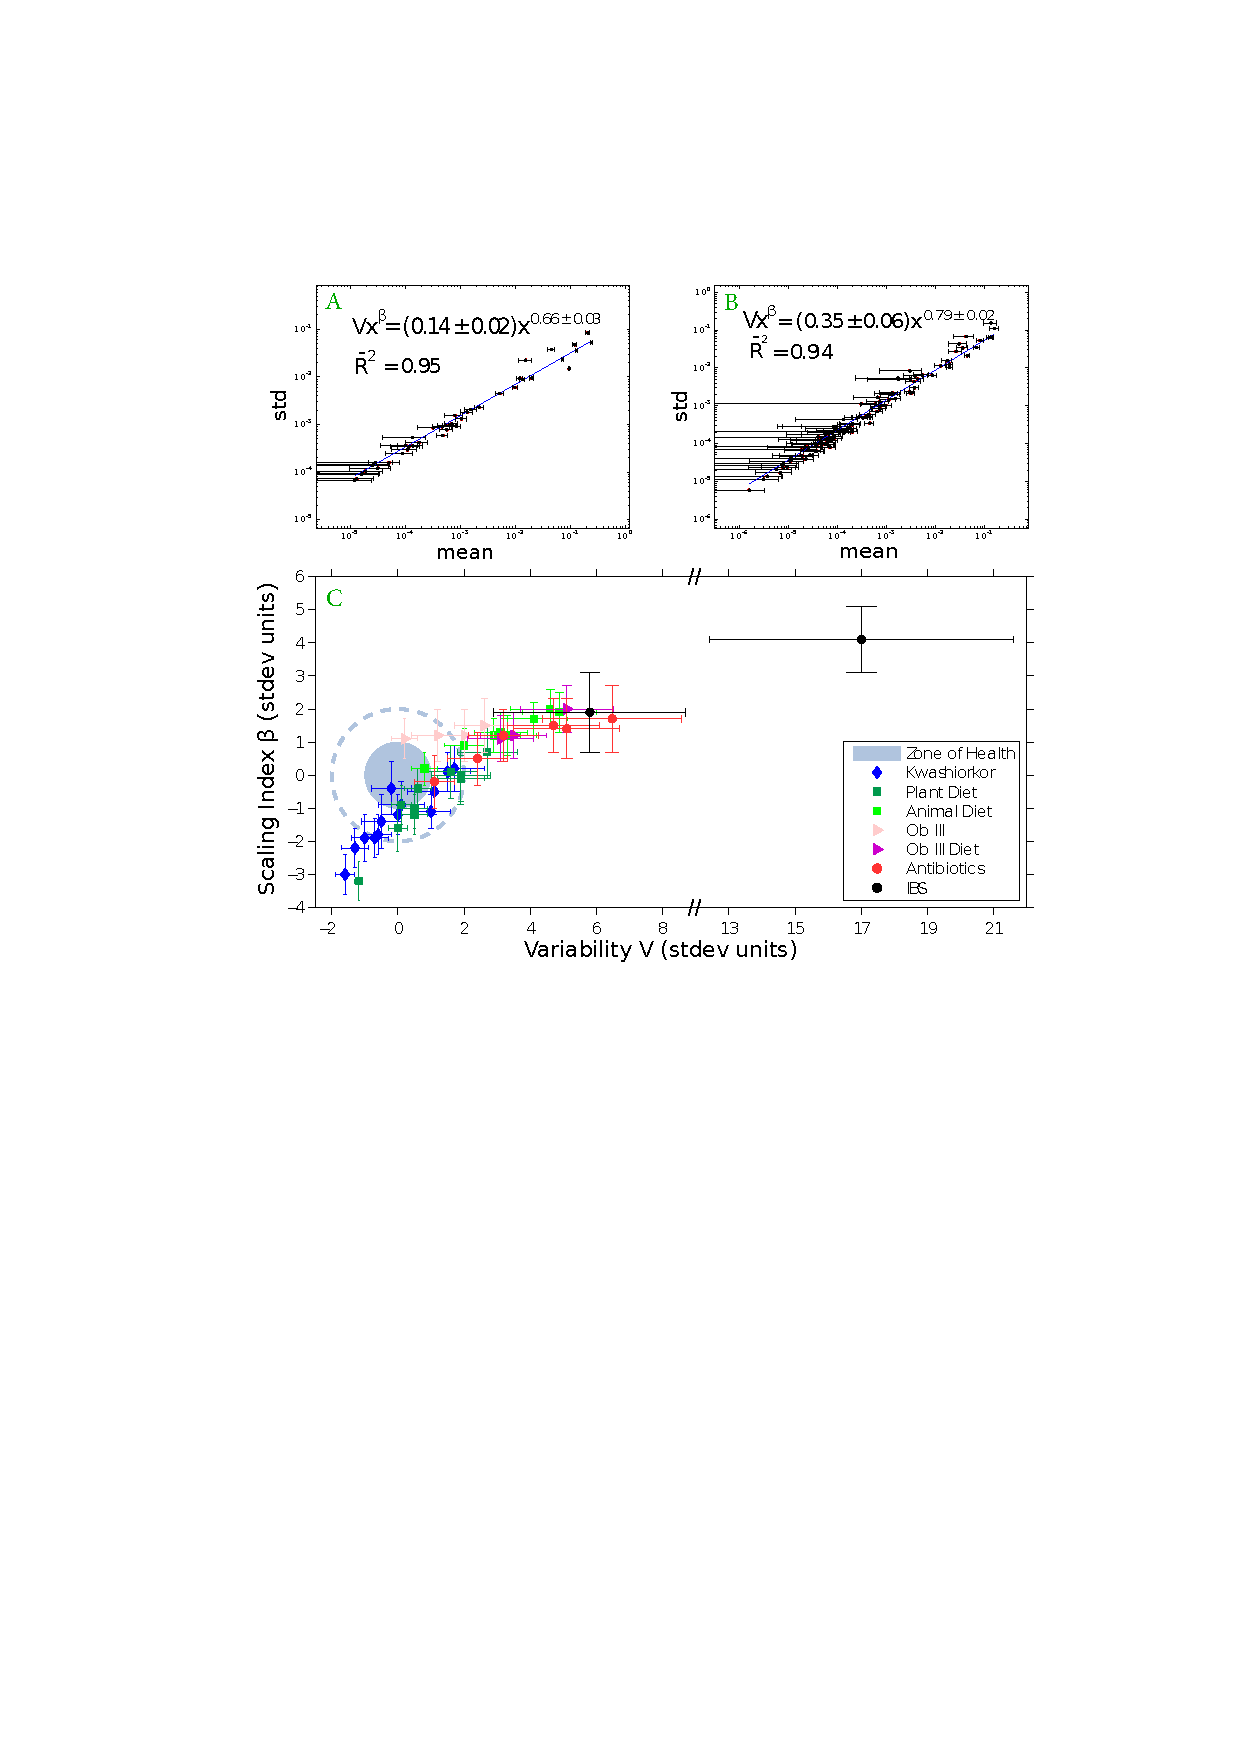
\includegraphics[width=1.05\textwidth]{comboplot1.pdf}
\caption{Taylor's law parameter space. X-weighted power-law fits of the standard deviations versus the mean values for each bacterial genus monitored in time. We show the fit for samples from a healthy subject (Fig. A) and from a subject diagnosed with irritable bowel syndrome (Fig. B) studied in our lab\cite{durban}. We have compiled all data studied in this work in Figure C. The coloured region (dashed line) corresponds to 68\% (95\%) CL region of healthy individuals in the Taylor parameter space. Points with errors place each individual gut microbiome in the Taylor space.}
\end{figure}


We have analysed the microbiome temporal variability to extract global properties of the system. As fluctuations in total counts are plagued by systematics errors, we worked with relative abundances. Our first finding was that, in all cases, changes in relative abundances of taxa follow a universal pattern known as the fluctuation scaling law\cite{fs} or Taylor's power law\cite{taylor}, i.e., microbiota of all detected taxa follows a power law dependence between mean relative abundance $x_i$ and dispersion $\sigma_i$, $\sigma_i  = V\cdot x_i^{\beta}$. While the law is universal, spanning six orders of magnitude in the observed relative abundances, the power law (or scaling) index $\beta$ and the variability $V$ (hereafter Taylor parameters) appear to be correlated with the stability of the community and the health status of the host (see Fig. 1). Our results hint at a universal behaviour. Firstly, the variability (which corresponds to the maximum amplitude of fluctuations) is large, which suggests resilient capacity of the microbiota, and the scaling index is always smaller than one, which means that, more abundant taxa are less volatile than less abundant ones. Secondly, Taylor parameters for the microbiome of healthy individuals in different studies are compatible within estimated errors. This enables us to define the health zone in the Taylor parameter space. We can better visualize the results of individuals from different studies by standardizing their Taylor parameters, where standardization means that each parameter is subtracted by the mean value and divided by the standard deviation of the group of healthy individuals in the study (see supplementary material). The zone of health and the standardized Taylor parameters for individuals whose gut microbiota is threatened (i.e., suffering from kwashiorkor, altered diet, antibiotics, IBS) is shown in Figure 1. Children developing kwashiorkor show smaller variability than their healthy twins. A meat/fish-based diet increases the variability significantly when compared to a plant-based diet. All other cases presented increased variability, which is particularly severe, and statistically significant at more than 95\% CL, for obese patients grade III on a diet, individuals taking antibiotics or IBS--diagnosed patients. A global property emerges from all worldwide data collected: Taylor parameters characterize the statistical behaviour of microbiome changes. Our conclusions are robust to systematic errors due to taxonomic assignment.

\begin{figure}[!ht]
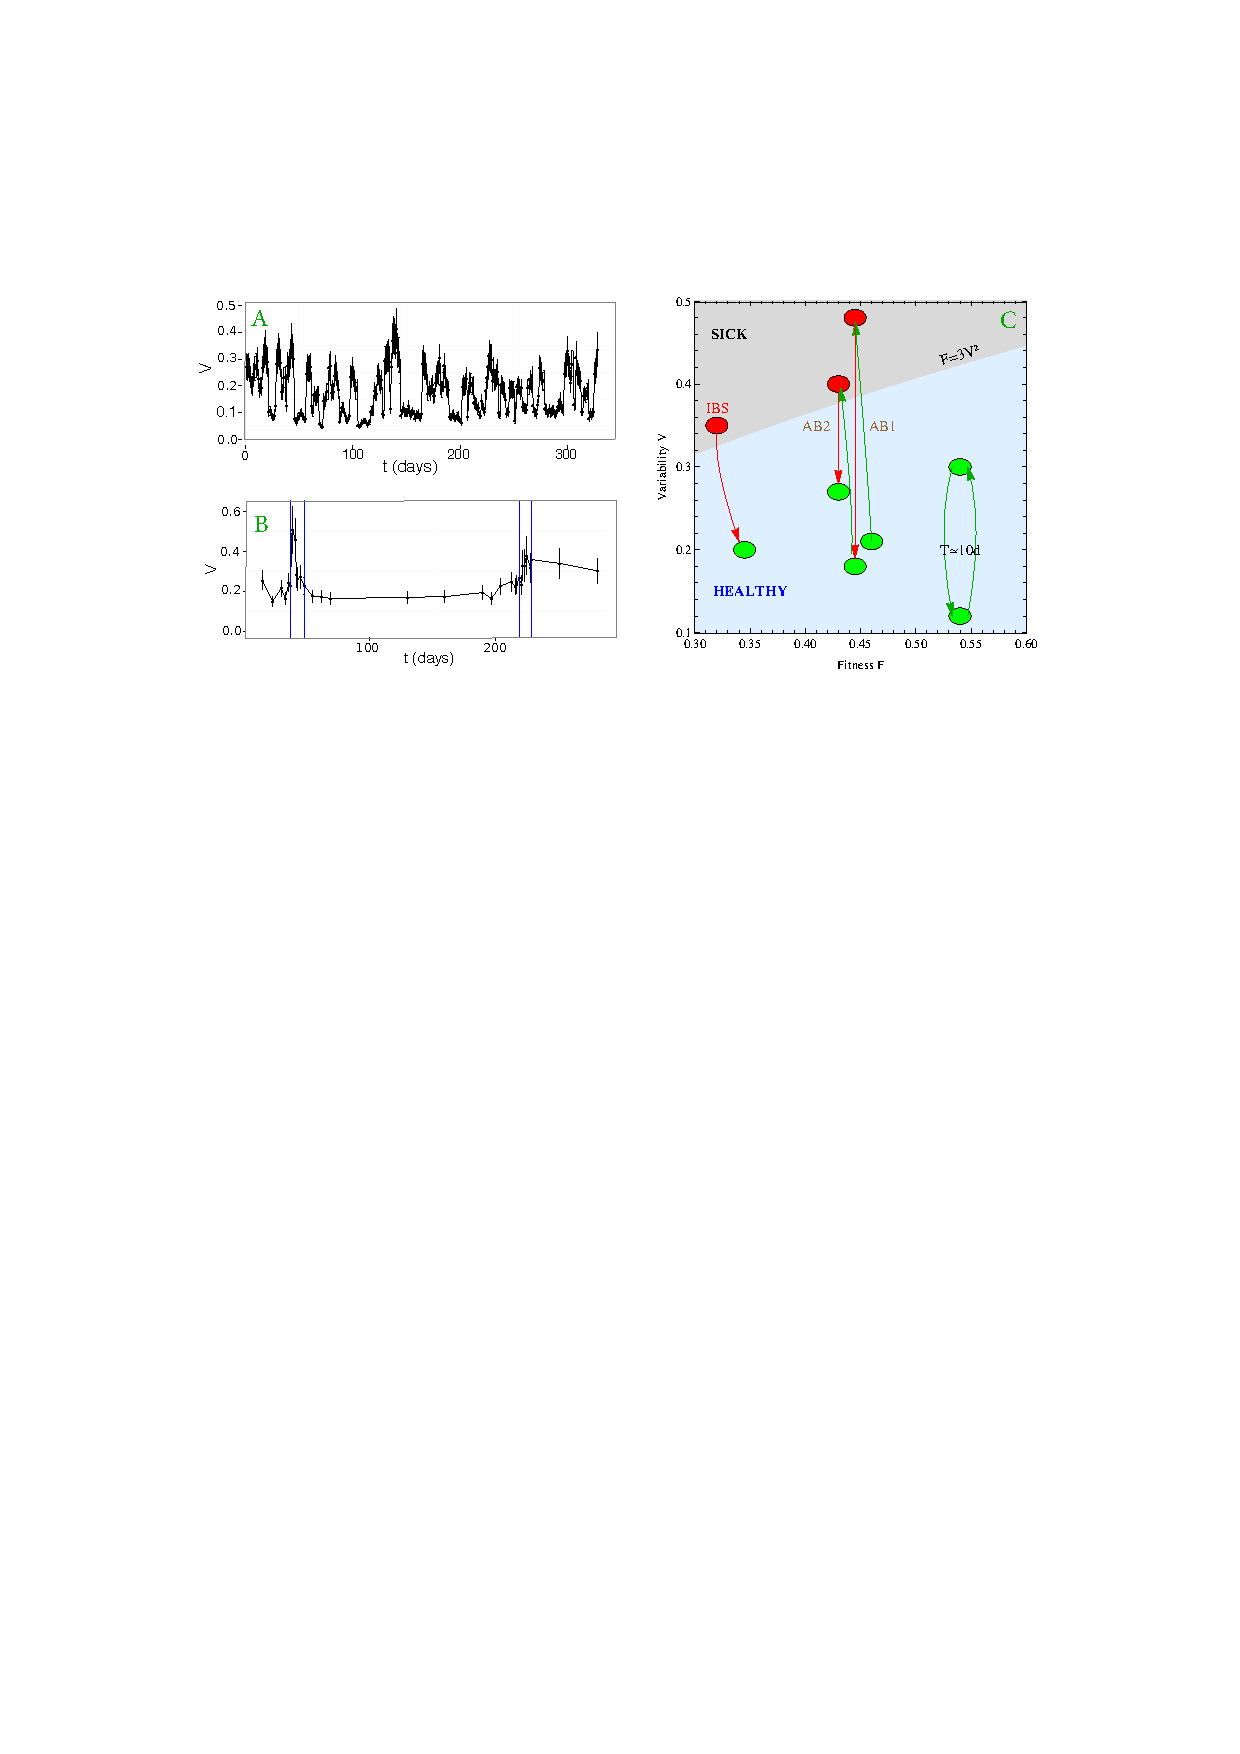
\includegraphics[width=1.05\textwidth]{comboplot2.pdf}
\caption{Phase space of microbiota stability. We show the Variability parameter as a function of time for the male in Caporaso's study\cite{moving} (Fig. A) and for the patient D in the antibiotics study\cite{antibiotic} (Fig. B). Periods of antibiotic treatment are shown by blue vertical lines. Microbiota states can be placed in the phase space F-V (Fig. C). The light blue (grey) shaded region corresponds to the stable (unstable) phase (the phase transition line is calculated for  $\alpha$ = $\beta$ = 0.75). We place healthy individuals (green) and individuals whose gut microbiota is threatened (antibiotics, IBS) in the phase space fitness - variability. Healthy individuals (green) show quasi-periodical variability. Individuals whose gut microbiota was threatened (red) show a phase transition to the healthy phase.}
\end{figure}

Taylor's power law has been explained in terms of various effects, all without general consensus. It can be shown to have its origin in a mathematical convergence similar to the central limit theorem, so virtually any statistical model designed to produce a Taylor law converge to a Tweedie distribution\cite{stat}, providing a mechanistic explanation based on the statistical theory of errors\cite{convergence1,convergence3}. We model the system by assuming that taxon relative abundance follows a Langevin equation with a deterministic term that captures the fitness of each taxon and a randomness term with Gaussian random noise\cite{ranking}. Both terms are modelled by power laws, with coefficients that can be interpreted as the taxon fitness $F_i$ and the variability $V$ (see Section 1 in supplemental material). Differences in variability $V$ can induce a noise-induced phase transition in relative abundances of taxa. The temporal evolution of the probability of a taxon having abundance $x_i$ given its fitness is governed by the Fokker--Planck equation. The results of solving this equation show that  the stability is best captured by fitness F and amplitude of fluctuations V phase space (see Fig. 2). 
The model predicts two phases for the gut microbiome: a stable phase with large variability that permits some changes in the relative abundances of taxa and an unstable phase with larger variability, above the phase transition, where the order of abundant taxa varies significantly with time. The microbiome of all healthy individuals was found to be in the stable phase, while the microbiome of several other individuals was shown to be in the unstable phase. In particular, individuals taking antibiotics and IBS--diagnosed patient P2 had the most severe symptoms. In this phase diagram, each microbiota state is represented by a point at its measured variability V and inferred fitness F. The model predicts high average fitness for all taxa, i.e., taxa are narrowly distributed in F. The fitness parameter has been chosen with different values for demonstrative purposes. Fitness is larger for the healthiest subjects and smaller for the IBS--diagnosed patients.  

In summary, we have quantitatively characterized whether the microbiota belongs to a healthy individual or a subject corresponding to an altered or pathological state (ie, altered diet, antibiotic treatment, early gut development, diagnosed IBS). Deciphering the mechanisms of disease requires in depth knowledge of the underlying biological mechanisms. We describe here the macroscopic behavior of disease by a noise-induced phase transition with a control parameter that can be measured by the temporal variability of the microbiome. The microbiota of healthy individuals and of individuals with pathologies represent different phases separated by this noise-induced phase transition. Improved high--throughput sequencing of samples from individuals monitored over time and taxonomic assigning methods will provide a better distinction among pathologies or altered states of the microbiota. 


\begin{thebibliography}{1}
\bibitem{moving} Caporaso, J.G. \textit{et al.} {\it Genome Biol.} {\bf 12,} R50 (2011).
\bibitem{lea} Faith, J.J. \textit{et al.} {\it Science} {\bf 341,} 1237439 (2013).
\bibitem{kwashiorkor} Smith M.I. \textit{et al.} {\it Science} {\bf 339,} 548-54 (2013).
\bibitem{diet} David, L.A. \textit{et al.} {\it Nature} {\bf 505,} 559-63 (2014).
\bibitem{antibiotic} Dethlefsen L., Relman D.A. {\it Proc. Nat. Acad. Sci. USA} {\bf 108,} 4554-61 (2011).
\bibitem{durban} Durban, A. \textit{et al.} {\it FEMS Microbiol. Ecol.} {\bf 86}, 581-9 (2013).
\bibitem{qiime} Caporaso, J.G. \textit{et al.} {\it Nature Methods} {\bf 7,} 335-6 (2010).
\bibitem{lmat1} Ames, S.K. \textit{et al.} {\it Bioinformatics} {\bf 29,} 2253-2260 (2013).
\bibitem{lmat2} Ames, S.K. \textit{et al.} {\it Genome Research} {doi:10.1101/gr.184879.114} (2015).
\bibitem{fs} Eisler, Z., Bartos, I., Kertesz, J. {\it Adv. Phys.} {\bf 57,} 85 (2008).
\bibitem{taylor} Taylor, L.R. {\it Nature} {\bf 189,} 732-35 (1961).
\bibitem{stat} Jorgensen, B., Martinez, J.R. {\it Scand. J. Statist..} {\bf 21,} 223-243 (1994).
\bibitem{convergence1} Fronczak, A., Fronczak, P. {\it Phys. Rev. E} {\bf 81,} 066112 (2010).
\bibitem{convergence3} Kendal, W.S., Jorgensen, B. {\it Phys. Rev. E} {\bf 84,} 066120 (2011).
\bibitem{ranking} Blumm, N. \textit{et al.} {\it Phys. Rev. Lett.} {\bf 109,} 128701 (2012).
\end{thebibliography}

\end{document}




